\chapter{Results}\label{chapter:results}
In this chapter, we present the results of our experiments.
Starting with an evaluation of the retrieval pipelines, we follow with showing the effectiveness of the different LLMs on the rank-based implicit evaluation method.
The results and visualizations needed to evaluate the research questions formulated in the Introduction are presented.

\section{Evaluation of Retrieval Pipelines}
In this section, we compare the effectiveness of the different retrieval pipelines.
We chose to evaluate the pipelines using nDCG@10.
nDCG is a suitable metric for our task, as it takes into account multiple different relevance/credibility/readability levels instead of only the binary relevant/non-relevant distinction.
Furthermore, it emphasizes the importance of the pipeline being able to distinguish between answers at the top level by giving more weight to the top results.
We chose a cutoff of 10 because even though the minimum available number of answers per query is 39, the number of relevant results is much lower.
This also normalizes the rank position between the different queries, as the number of assessed documents per query varies.
\begin{table}[tb]
\centering
\begin{tabularx}{\textwidth}{lXXX}
\hline
Pipeline    & Relevance          & Readability        & Credibility        \\ \hline
DPH         & 0.643 & 0.742 & 0.539 \\
DPH\ (qe)     & 0.637 & 0.751 & 0.51  \\
TF-IDF     & 0.64  & 0.746 & 0.551 \\
TF-IDF (qe) & 0.636 & 0.751 & 0.557 \\
ColBERTv1      & 0.626 & 0.774 & 0.633 \\
ColBERTv2       & 0.634 & 0.799 & 0.65  \\
duoT5            & 0.64  & 0.805 & 0.714 \\
monoT5           & \textbf{0.645} & \textbf{0.813} & \textbf{0.722} \\
\hline
\end{tabularx}
\caption{Results of the transformer pipelines, shown as nDCG@10. The best results of the baseline pipelines are shown for comparison. All models are trained on the MS MARCO passage ranking dataset (\cite{bajaj:2016:MSMARCO}).}
\label{tab:transformer_pipelines}
\end{table}
\subsection{Baseline Pipelines}
Our baseline retrieval pipelines are the TF-IDF and BM25 pipelines, each once with and once without query expansion.
Effectiveness on all three dimensions is similar for all pipelines, showing little difference between the strategies.
Table \ref{tab:transformer_pipelines} shows the retrieval effectiveness of the baseline pipelines in the first four rows.
The rankings are closest to the human rankings for readability, scoring around 0.75 for all pipelines.
Relevance is lower than that, with scores around 0.64.
Since those models are designed to retrieve relevant documents, we would expect the relevance scores to be higher.
The credibility scores are the lowest, with scores around 0.55.

\subsection{Transformer Pipelines}
Table \ref{tab:transformer_pipelines} shows the nDCG@10 scores for the different transformer-based pipelines, compared to the best baseline results.
The monoT5 pipeline is most effective on all three dimensions, with scores of 0.645 for relevance, 0.813 for readability, and 0.722 for credibility.
Re-ranking the top 10 results using duoT5 made the results slightly worse in all dimensions.
ColBERTv2 shows a slight improvement over ColBERTv1 but is still worse in relevance while being better in readability and credibility.

In general, the transformer-based models have very similarly effectiveness to the baseline models in terms of ranking for relevance, but all transformer-based models achieve higher scores on readability and credibility.

\subsection{External Document Scores}
To investigate if adding external scores to the ranking process could improve the document rankings, we calculate statistical readability scores for all documents in the dataset.
We then compare the calculated scores to the readability scores assigned by the human annotators.
For our dataset, we do not find a strong correlation between the human-annotated readability scores and the statistical scores.
The Flesch Reading Ease score has a correlation of 0.177 with the readability scores, while the full textstat score has a slightly negative correlation of -0.147.
Those correlations are not strong enough to justify using the statistical scores as a proxy for readability.

This might be connected to the fact that the documents in our dataset are scraped from the web, which means that even after preprocessing they still contain noise not accounted for by the statistical scores, which are intended for the use on clean text.

\subsection{Summary}
Because monoT5 is most effective on ranking in all three dimensions, we use it for all further experiments and only evaluate the one ranking produced by this pipeline.

We evaluate the LLM answer effectiveness on their normalized position, which is the absolute position of the answer in the ranking, divided by the total number of documents for the query.
\begin{equation}
    \text{Normalized Position} = \frac{\text{Absolute Position}}{\text{Total Number of Documents for Query}}
\end{equation}

\section{Factors influencing LLM effectiveness}
In this section, we present results that help in investigating how different factors affect the effectiveness of health answers by LLMs on the implicit evaluation method.
We look at the influence of model size, prompting strategy, answer length and query type on the ranking of the LLM answers.
Additionally, we investigate the answers generated by ChatGPT that are ranked especially low.

In total, we rank 16000 generated answers, with each of the 8 models generating 10 answers for the 4 different prompting strategies for all 50 queries.
\begin{figure}[tb]
\centering
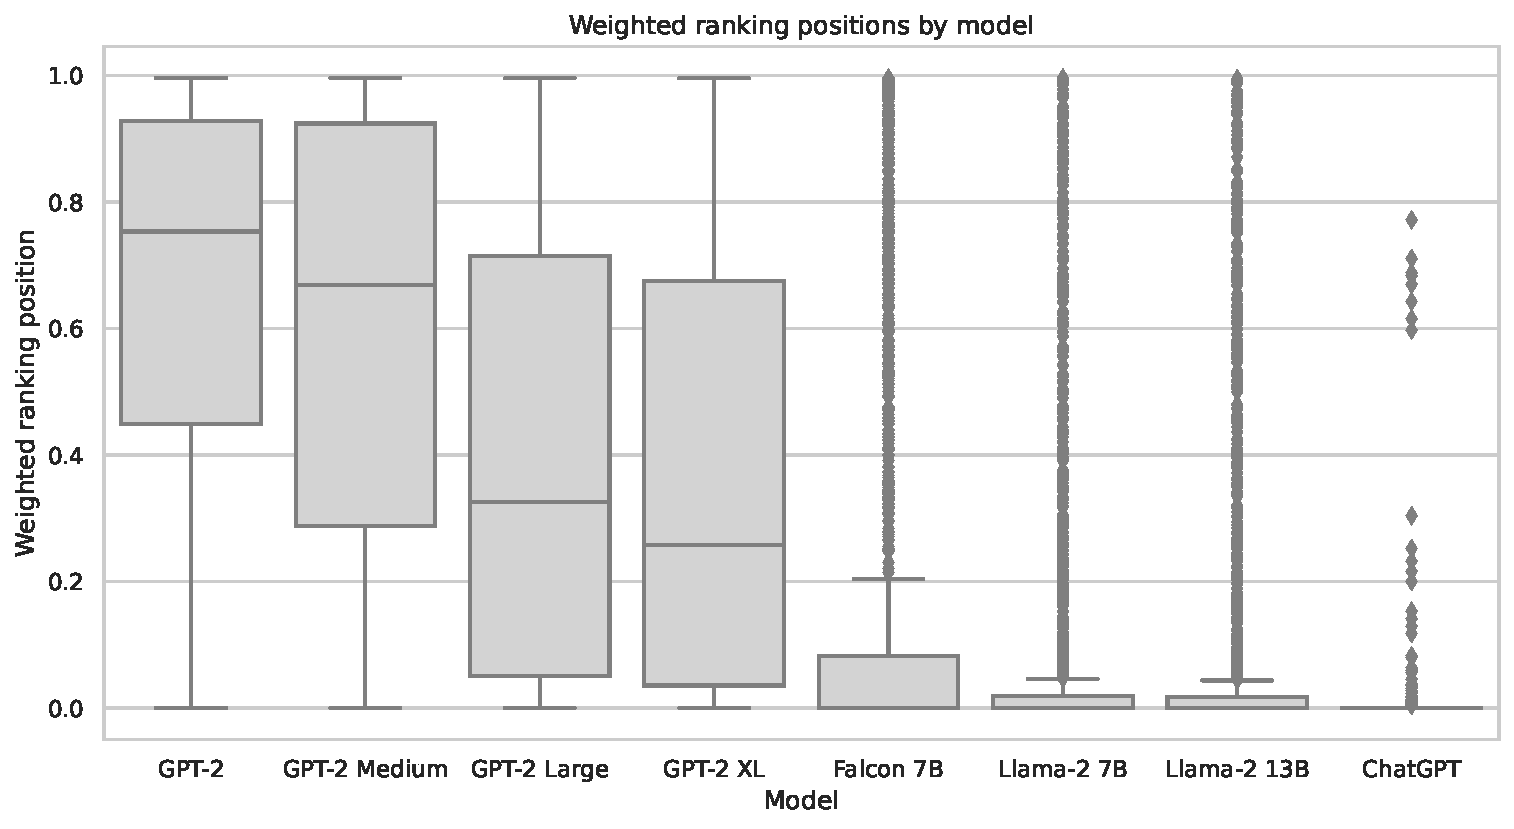
\includegraphics[width=\textwidth]{images/weighted_position_boxplot.pdf}
\caption{Boxplot of the normalized position of the LLM answers by model. The normalized position is the absolute position of the answer in the ranking, divided by the total number of documents for the query.}
\label{fig:weighted_position_boxplot}
\end{figure}
Figure \ref{fig:weighted_position_boxplot} shows the normalized position of the LLM answers in the ranking.

Of all models, ChatGPT is most effective with a median normalized position of 0.006, scoring the best or second-best answer at nearly all queries.
Falcon 7B is the worst of the fine-tuned models with the Llama models being slightly more effective.
The GPT-2 models show the lowest rankings overall, but show a clear trend of better rankings with increasing model size.

All models show a large spread in the rankings, with the most effective models generally having a smaller spread.
ChatGPT is the most consistent model, with the smallest standard deviation of 0.05.
The other models have much higher standard deviations, with the Llama models both being around 0.2 and the other models between 0.3 and 0.35.

The spread of all GPT-2 models is so large that the 0.25 and 0.75 quantiles overlap with the minimum and maximum values, showing the consistently large spread of answer rankings for those models.
Even though the spread between the 0.25 and 0.75 quantiles is smaller for the fine-tuned models, all of them still have outliers towards the bottom of the ranking.


\subsection{Influence of Model Size}
\begin{figure}
    \centering
    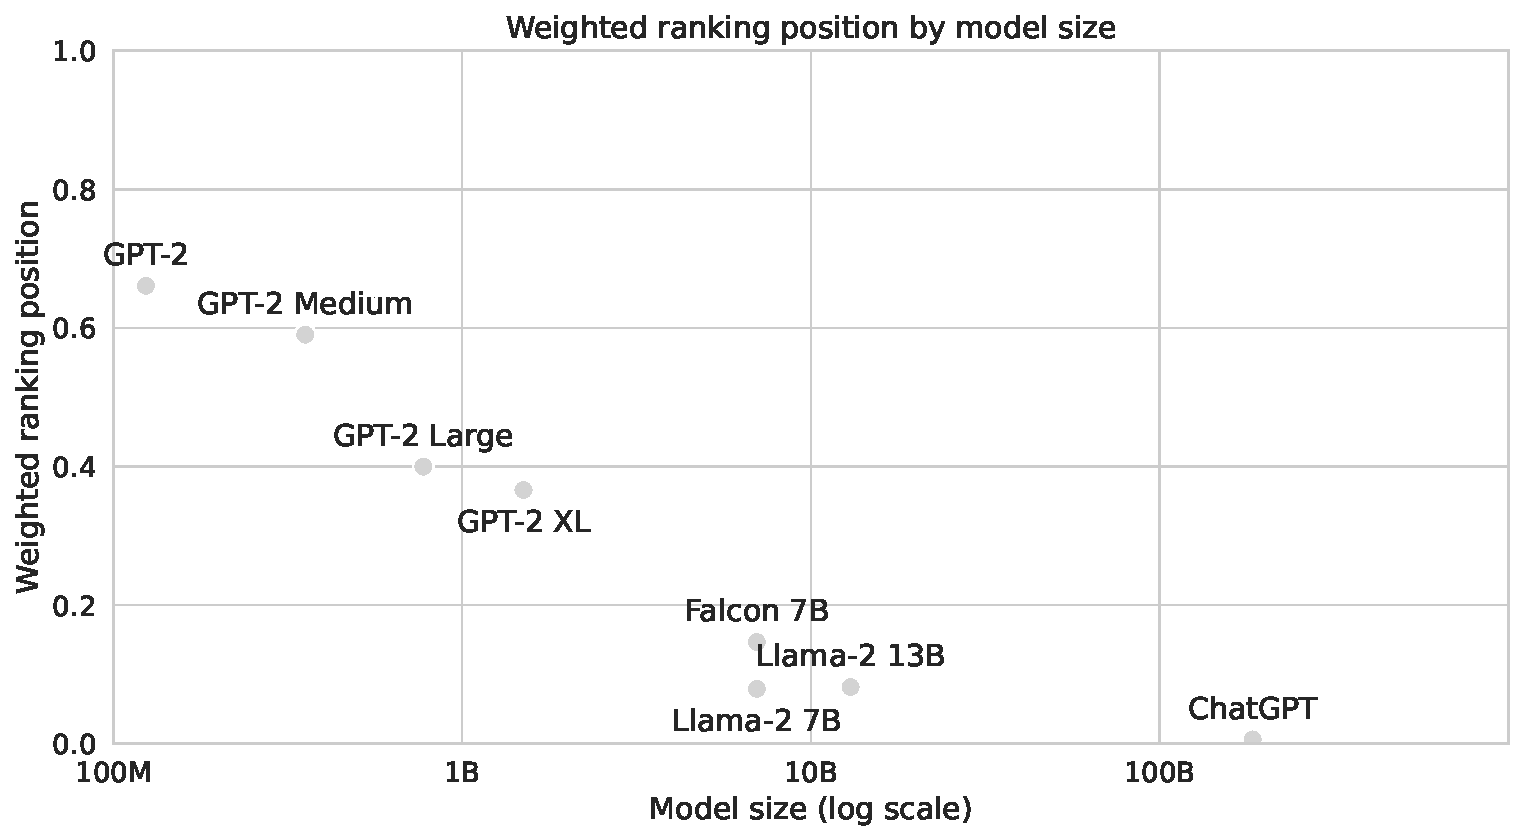
\includegraphics[width=\textwidth]{images/weighted_position_vs_model_size.pdf}
    \caption{Scatterplot showing number of model parameters against weighted normalized position of the model answers, as the mean over all prompts. Model size is shown on a logarithmic scale.}
    \label{fig:weighted_position_vs_model_size}
\end{figure}

Figure \ref{fig:weighted_position_vs_model_size} shows the weighted normalized position of the LLM answers plotted against the number of model parameters.
There is a clear trend of more model parameters leading to better rankings, with the GPT-2 models generating the least effective answers and the 185B parameters ChatGPT model generating the most effective answers.
The improvement is not linear, with the biggest improvements happening between GPT-2 Medium and GPT-2 Large, and between GPT-2 XL and Falcon 7B/Llama-2 7B.


\subsection{Influence of Prompting Strategy}
\begin{table}[tb]
\centering
\begin{tabular}{lllll}
\hline
\textbf{Model}        & \textbf{No Prompt} & \textbf{QA}     & \textbf{QuestionAnswer} & \textbf{MultiMedQA} \\\hline
GPT-2        & 0.763      & 0.663 & 0.614    & \textbf{0.603}      \\
GPT-2 Medium & 0.675      & \textbf{0.524} & 0.544    & 0.618      \\
GPT-2 Large  & 0.496      & 0.393 & \textbf{0.336}    & 0.374      \\
GPT-2 XL     & 0.509      & 0.336 & 0.327    & \textbf{0.292}      \\
Falcon 7B    & 0.324      & 0.133 & 0.118    & \textbf{0.012}      \\
Llama-2 7B   & 0.211      & 0.073 & 0.027    & \textbf{0.005}      \\
Llama-2 13B  & 0.218      & 0.068 & 0.032    & \textbf{0.01 }      \\
ChatGPT      & 0.006      & 0.01  & 0.007    & \textbf{0.001}     \\
\hline
\end{tabular}
\caption{Mean normalized position of the LLM answers, by prompting strategy.
The most effective prompting strategy to generate answers for each model is highlighted in bold.
The prompting strategies are described in section \ref{sec:prompting-approaches}, order here from least to most complex.
Increasing prompting complexity generally improves the ranking of the LLM answers for most models, with exception to GPT-2 Medium and GPT-2 Large.
}
\label{tab:prompting_strategy}
\end{table}
The different prompting strategies strongly influence the final rankings of the LLM answers.
Table \ref{tab:prompting_strategy} shows the mean normalized position of the LLM answers for the different prompting strategies.
Starting with no prompt produces the worst ranking results for all models, except for ChatGPT where the QuestionAnswer prompt is slightly less effective.
The rankings improve with each more complex prompting strategy, except for GPT-2 Medium and GPT-2 Large, which is most effective on the QA and the QuestionAnswer prompts respectively.
For all other models, the ranking is best on the complex MultiMedQA prompt.

Inside each prompting strategy, the ordering of the models is consistent except for the Llama models, which change between second and third place depending on the prompting strategy.

\subsection{Keyword vs Question Queries}
\begin{figure}
    \centering
    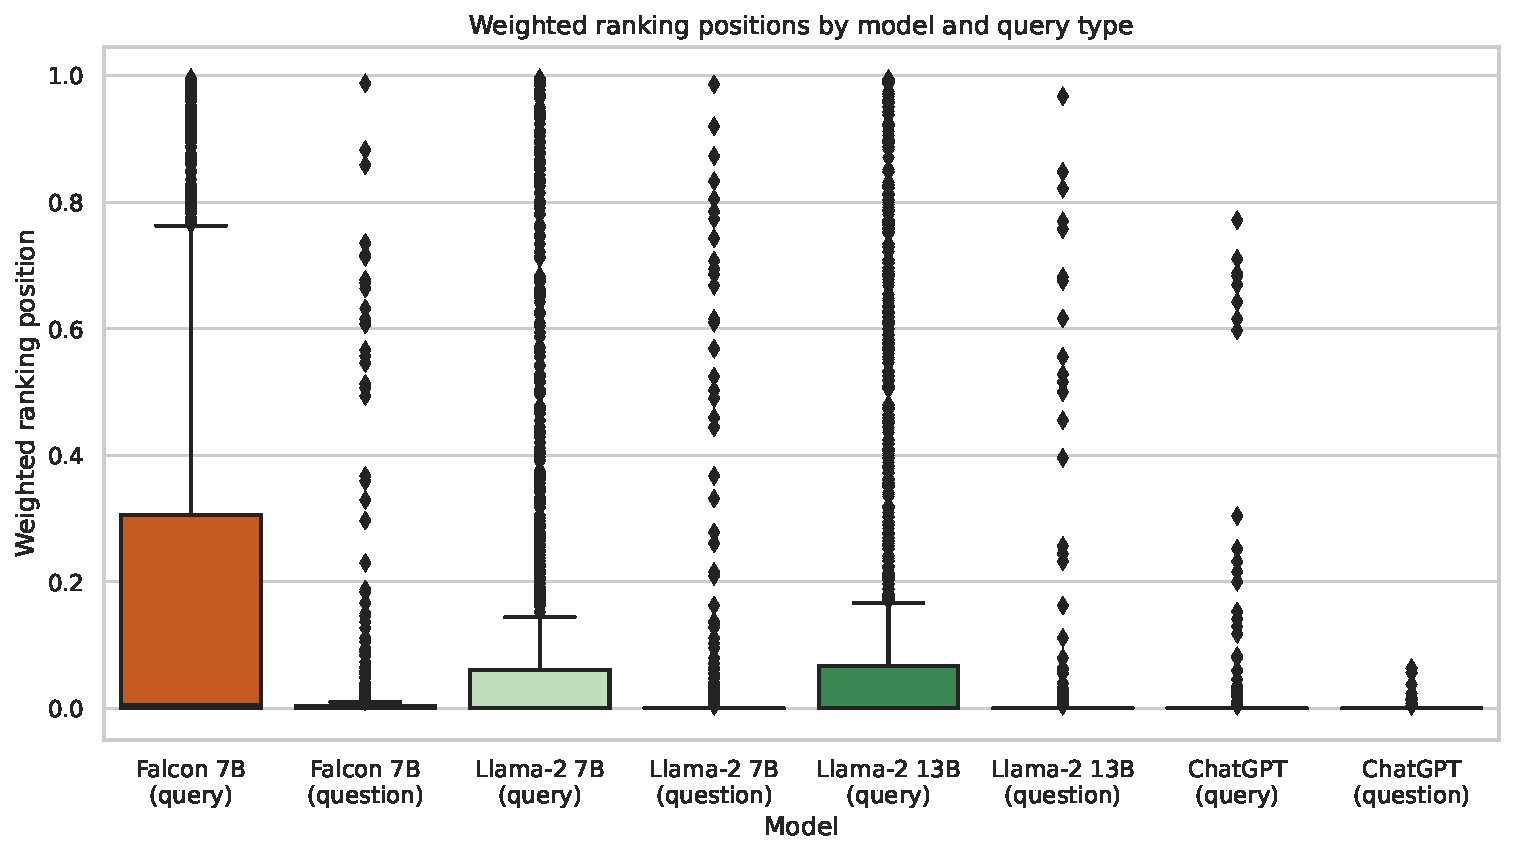
\includegraphics[width=\textwidth]{images/weighted_position_boxplot_by_model_and_question.pdf}
    \caption{Boxplot of the normalized position of the LLM answers, by model and query type.}
    \label{fig:weighted_position_boxplot_by_model_and_question}
\end{figure}
Figure \ref{fig:weighted_position_boxplot_by_model_and_question} shows the normalized position of the LLM answers, split by query type and model.
Question-type queries are identified by the last character of the query being a question mark, while keyword queries are all other queries.
Answers generated for the properly phrased question-type queries achieve higher median rankings than the answers generated for the keyword queries.
The spread of the rankings is also smaller for the question-type queries, with the keyword queries having more outliers at the bottom of the ranking.
This also holds true for ChatGPT, which is the most consistent model overall.
The GPT-2 based models exhibit the same pattern of question-type queries being ranked better than keyword queries, but are omitted from Figure \ref{fig:weighted_position_boxplot_by_model_and_question} for better readability.

\subsection{Lower Ranked ChatGPT Answers}
While ChatGPT generally provides the most effective answers, there are still some answers that are ranked poorly.
We manually inspect each of the ChatGPT generated answers with a normalized ranking position of 0.1 or higher, meaning if there are 100 documents for the query, the answer is ranked 10 or lower.
All the low ranked answers stem from four queries, namely ``hypothyroidism symptoms'', ``List of multiple sclerosis symptoms'',  ``exercises for better posture'' and ``my risk for developing type 2 diabetes'' and follow one of two patterns.
The answers for the question about the personal risk of developing type 2 diabetes all contain the phrase ``As an AI'', as in the phrase ``I'm sorry, but as an AI language model, I don't have access to personal data about individuals unless it has been shared with me in the course of our conversation.''.
This is a commonly used phrase by ChatGPT, which indicates that the model is unable to answer the question.
The answers for the other three queries are all formatted as lists, either using enumeration or simple bullet points.
To investigate if answers formatted as lists are generally ranked lower, we identify all answers that are formatted as lists by searching for generated answers containing more than five non-empty lines, of which at least three start with either a dash or a number.
We also identify all answers containing the phrase ``As an AI''.
Table \ref{tab:badly_ranked_answers} shows the mean normalized ranking position of the LLM answers, split by whether they are formatted as lists.
\begin{table}[tb]
    \centering
    \begin{tabular}{lcc}
    \hline
    \textbf{Models} & \multicolumn{2}{c}{\textbf{List Style}} \\
    \cline{2-3} 
    & \textbf{Yes} & \textbf{No} \\
    \hline
    \multirow{2}{*}{GPT-2}        & N/A           & 0.6608  \\
                                  & (0)           & (2000) \\
    \multirow{2}{*}{GPT-2 Medium} & N/A           & 0.5902  \\
                                  & (0)           & (2000) \\
    \multirow{2}{*}{GPT-2 Large}  & 0.4365        & 0.3992  \\
                                  & (36)          & (1964) \\
    \multirow{2}{*}{GPT-2 XL}     & 0.4004        & 0.3658   \\
                                  & (22)          & (1978)  \\
    \multirow{2}{*}{Falcon 7B}    & 0.312         & 0.1436  \\
                                  & (38)          & (1962) \\
    \multirow{2}{*}{Llama-2 7B}   & 0.0416        & 0.0849  \\
                                  & (266)         & (1734) \\
    \multirow{2}{*}{Llama-2 13B}  & 0.0483        & 0.0909  \\
                                  & (427)         & (1573) \\
    \multirow{2}{*}{ChatGPT}      & 0.0128        & 0.0021  \\
                                  & (748)         & (1252) \\
    \hline
    \end{tabular}
    \caption{Mean normalized ranking position of the LLM answers, split by whether they are formatted as a list. The number in brackets is the number of answers in that category. If that number is 0, the model did not generate any answers in that format, so the mean is not available (N/A).}

    \label{tab:badly_ranked_answers}
\end{table}
ChatGPT generates the most answers formatted as lists, with 748 of the 2000 answers following that pattern.
On average, those answers are ranked worse than the other answers by ChatGPT, with a mean normalized ranking position of 0.0128 compared to 0.0021 for the non list answers.
The other models do not generate as many answers formatted as lists, with the both Llama models generating the most, 427 and 266 respectively.
The answers by the Llama models which are formatted as lists score higher than the non-list ones, while for the remaining models the answer rank follows the ChatGPT pattern, in that list-style answers are ranked lower than non list-style answers.

For ChatGPT, the answers containing the phrase ``As an AI'' are ranked worse than the other answers, with a mean normalized ranking position of 0.0578 compared to 0.0056.
They are also generated less frequently, with only 20 of the 2000 answers containing the phrase.
The only other model generating that phrase is the Falcon 7B model, which generates it 30 times.
With a mean normalized rank of 0.191 the answers containing the phrase also rank worse, but the difference is not as pronounced compared to the rank of 0.146 which the remaining answers by Falcon 7B achieve.

\subsection{Influence of Answer Length}
\begin{figure}
    \centering
    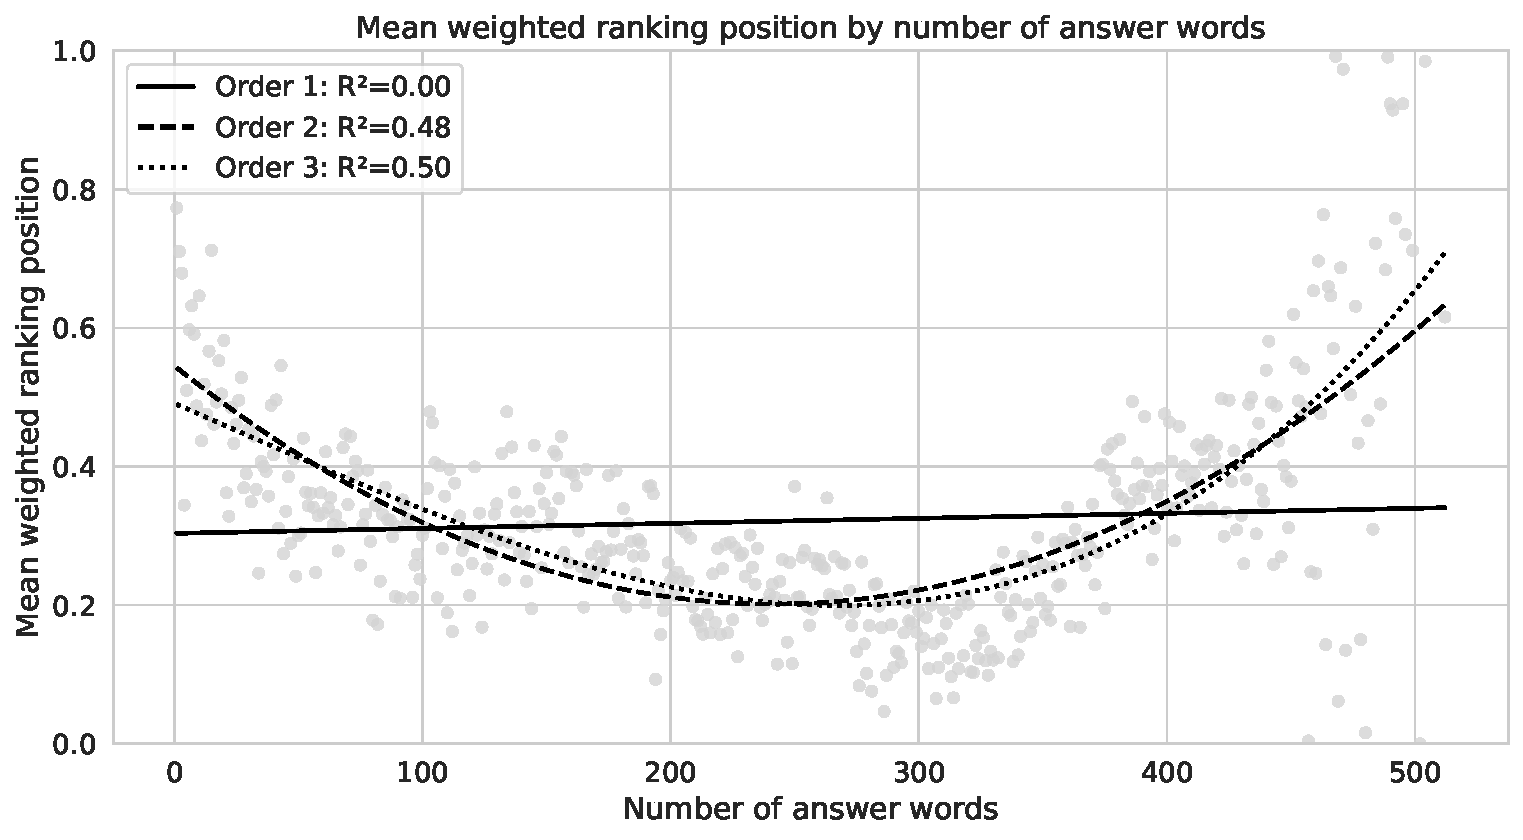
\includegraphics[width=\textwidth]{images/weighted_position_vs_num_answer_words.pdf}
    \caption{Scatterplot showing the weighted normalized position of the LLM answers against the number of words in the answer. 
    To improve visibility, we show the mean of the weighted normalized position for each answer length, so the standard deviation is not visible.
     Three regression lines of order 1, 2 and 3 are shown.}
    \label{fig:weighted_position_vs_answer_length}
\end{figure}
We investigate the influence of answer length on the ranking of the LLM answers by plotting the weighted normalized position against the number of words in the answer.
Figure \ref{fig:weighted_position_vs_answer_length} shows the scatterplot of the weighted normalized position against the number of words in the answer, with three regression lines which are linear (order 1), quadratic (order 2) and cubic (order 3).
The linear regression fails to capture the variance in the data, indicated by the R-squared value of 0.
With R-squared values of 0.48 and 0.50, the quadratic and cubic regression lines are better at capturing the variance, indicating a parabolic relationship between answer length and ranking.
Very short and long answers are ranked worse than answers of medium length, with the best ranking answers on average having between 200 and 350 words.
Of the 3271 answers with more than 350, about 85\% are generated by any of the GPT-2 models.
Manual evaluation shows that many of the answers show a pattern of repeating the same phrase multiple times, leading to a high word count but not adding any additional information to the answer.

\section{Comparison to other Benchmarks}\label{sec:benchmark_comparison}
We compare the median normalized ranking position of the LLM answers to the results of other benchmarks.
To our knowledge, there are currently no benchmarks available that evaluate the effectiveness of LLMs for LFQA and provide results for the same models that we use.
The HuggingFace Open LLM Leaderboard by \cite{beeching:2023:Open} provides results on multiple different benchmarks for many models hosted on the HuggingFace hub.
From here, we select the ARC~(\cite{clark:2018:Think}), the HellaSwag~(\cite{zellers:2019:HellaSwag}) and the MMLU~(\cite{hendrycks:2020:Measuring}) datasets, all of which are single choice question answering benchmarks.
\begin{table}[tb]
    \centering
    \begin{tabularx}{\textwidth}{lcccc}
    \hline
    \textbf{Model} & \textbf{Mean Ranking} & \textbf{ARC}  & \textbf{HellaSwag} & \textbf{MMLU} \\\hline
    GPT-2          & 0.661                             & 21.8          & 31.6               & 25.9          \\
    GPT-2 Medium   & 0.59                              & 27.0          & 40.2               & 26.6          \\
    GPT-2 Large    & 0.4                               & 25.9          & 45.6               & 26.1          \\
    GPT-2 XL       & 0.366                             & 30.3          & 51.4               & 26.4          \\
    Falcon 7B      & 0.147                             & 46.2          & 70.9               & 25.8          \\
    Llama-2 7B     & 0.079                             & 52.9          & 78.6               & 48.3          \\
    Llama-2 13B    & 0.082                             & 59.0          & 81.9               & 54.6          \\
    ChatGPT        & \textbf{0.006}                    & \textbf{85.2} & \textbf{85.5}      & \textbf{70.0} \\
    \hline
    \end{tabularx}
    \caption{Comparison of the mean normalized ranking position of the LLM answers to the results of other benchmarks.
    For the HuggingFace models, those scores are taken from the HuggingFace Open LLM Leaderboard by \cite{beeching:2023:Open}.
    For ChatGPT, we estimate the score from the GPT-4 Technical Report~(\cite{openai:2023:GPT}), which provides scores for GPT-3.5, the underlying model of ChatGPT.
    This is not the exact model we use in out testing, but we assume that the capabilities are similar.
    Mean Ranking is the mean normalized ranking position over all generated answers for the model.
    }
    \label{tab:benchmark_comparison}
\end{table}
Table \ref{tab:benchmark_comparison} shows the scores over those benchmarks, as well as the mean normalized ranking position of the LLM answers.
On all benchmarks, there is the general trend of higher number of model parameters leading to better scores.
For our dataset this trend is only broken for the two Llama versions, with the 7B model ranking slightly better than the 13B model.
